%\chapter{USSS toolkits}
%shown in figure~\ref{fig:artificialnatural}
%pages~\pageref{tab:opposites1}
%and form (section~\ref{section:form}, page~\pageref{section:form}).

\chapter{Lesson plan}
\label{lessonplan}


\section{Scoring simple tunes}

\subsection{The triangle of film}
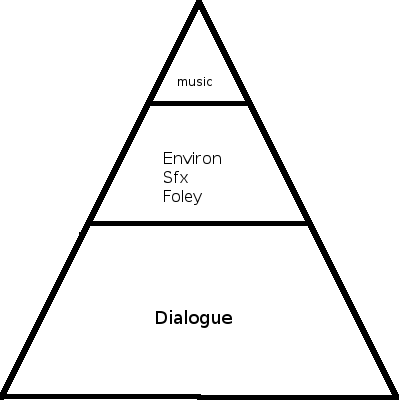
\includegraphics[scale=2.0]{triangleoffilm} 

\subsection{Simple examples}
\begin{itemize}
\item Melodic writing eg. Married life video from `Up' (a waltz in the original)
\item Score a simple melody for 16 bars. Analyse and feedback
\item Star Wars (Throne room scene: A march)
\item Examples: John Carter (2012, Stanton, music - Giacchino)
\end{itemize}

\subsection{Bring me sunshine} 
\begin{itemize}
\item Sunshine (Danny Boyle - 2007) clip 
\item Spot a piece of music from Naxos 
\item eg. Brahms1 (perhaps useful to quickly score in Sibelius and MuseScore) 
\item Add video (talk about music with video in Cubase, Premiere)
\item Introducing spotting music to clips and familiarity with Sibelius and/or MuseScore
\end{itemize}


\subsection{More spotting}
\begin{itemize}
\item Gladiator (Title 1, chapter 2 - battle scene) eg. spot with Holst Mars / compare original
\item Compose to the `battle' clip - piano only
\end{itemize}

\subsection{Harmony}
\begin{itemize}
\item Short score
\item 8 part orchestral sketch
\item Barber adagio for strings (Platoon, Stone)
\item Modes
\end{itemize}

\section{Orchestration}
\begin{itemize}
\item Woodwind (Stravinsky); Brass (Janacek, Copland): Copy in MuseScore
\item Examples. Vertigo (1958, Hitchcock - Hermann); Scott of the Antarctic (1948, Vaughan Williams); 
\item Robin Hood 1938, Korngold score; 1991, Dir: Kevin Reynolds, Music - Michael Kamen; 2010, Dir. Ridley Scott, Music - Marc Streitenfeld  
\end{itemize}

\section{Sfx}
\begin{itemize}
\item Examples: Bourne sfx; Wall-e; THX1138

\end{itemize}

\section{Writing something more experimental}
\begin{itemize}
\item This assignment could involve the use of Cubase and a more sfx / electroacoustic piece
\item The film choice could therefore be potentially `atmospheric'
\item Students may wish to be introduced to the USSStoolkit and use basic granulation to generate texture
\item Students may wish to borrow portable recorders to make their own sfx/foley
\item Foley - to picture
\item ADR - In addition to understanding the reason for ADR, in some submissions it will be important to put some of the dialogue back using students' own voices. 
\item This assignment can also be a popular music track  
\item Examples: Clockwork Orange (1971, Wendy Carlos); Bladerunner (1982, Vangelis); Social Network (2010, Trent Reznor, Atticus Ross); Forbidden Planet (1956, Barron); The Birds (1963, Hitchcock, Sala and the Trautonium)
\end{itemize}

\section{Visual Music}
\begin{itemize}
\item Examples of AV pieces where (in many cases) the composer is also the video artist. 
\item Taking this forward, students may wish to look at Processing and Blender. 
\item GEM in puredata might be useful.
\item Examples: Brett Battey; Louise Harris
\end{itemize}

\section{Opportunities: really important}
\begin{itemize}
\item South Yorkshire Filmmakers Network \url{http://syfn.org/}
\item If considering taking an special project module or extended special project with film music scoring as an outcome, scoring to materials downloaded from the internet is not allowed. You MUST find a film maker and document your process. Therefore, syfn is the place to get involved. 
\end{itemize}

\section{FAQ}
\begin{itemize}
\item Q: can I record a live ensemble? Yes, but the logistics make this almost impossible. 
\item Q: if I rip the film, I lose the dialogue and sfx,. Will I lose marks for not putting them back in. A: No, but why would you not want to make your clip as perfect as possible. We are now teaching Foley and ADR so it should be possible to approach something fully functional.
\item Q: can I rip my favourite film? A: Yes, but it will potentially be useless to score to. Hollywood isn't great for finding something really creative to work with. Better to find a finished and complete `short' so you experience scoring the whole film. 
\item Q: can I work with a film maker? A: Yes. In fact, as this is a \textbf{requirement} for MUS3040 Special Project with film. Search for South Yorkshire Filmmakers Network (syfn.org) see above.
\end{itemize}



